\documentclass[11pt]{article}
\usepackage[utf8]{inputenc}
\usepackage[T1]{fontenc}
\usepackage[margin=1in]{geometry}
\usepackage{amsmath}
\usepackage{booktabs}
\usepackage{graphicx}
\usepackage[hidelinks]{hyperref}
\usepackage{xcolor}

% Every number quoted from a result: generated by make.py.
\newcommand{\points}{105}
\newcommand{\fgpOverHqa}{1.24$\times$}
\newcommand{\naiveOverHqa}{3.45$\times$}
\newcommand{\hqaSpeedup}{7.8$\times$}
\newcommand{\cuccaroFgpOverHqa}{0.73$\times$}
\newcommand{\attractionCuccaro}{4.04$\times$}
\newcommand{\attractionCuccaroRange}{1.32--8.86}
\newcommand{\attractionRandom}{1.18$\times$}
\newcommand{\attractionRandomRange}{1.14--1.31}
\newcommand{\uniformAlltoall}{1.00$\times$}
\newcommand{\fgpAlltoall}{1.31$\times$}
\newcommand{\uniformRing}{1.06$\times$}
\newcommand{\fgpRing}{1.91$\times$}
\newcommand{\uniformGrid}{1.04$\times$}
\newcommand{\fgpGrid}{1.60$\times$}
\newcommand{\uniformLine}{1.10$\times$}
\newcommand{\fgpLine}{1.76$\times$}
\newcommand{\breakEven}{1.4}
\newcommand{\slotSaving}{18\%}
\newcommand{\lookAheadSaving}{10\%}
\newcommand{\horizonSpread}{2\%}
\newcommand{\fgpSlowerOneChannelAll}{1.21$\times$}
\newcommand{\fgpSlowerOneChannelLine}{1.49$\times$}
\newcommand{\fgpUnlimitedAll}{0.96$\times$}
\newcommand{\naiveUnlimitedAll}{1.03$\times$}
\newcommand{\latencyMeanBest}{12\%}
\newcommand{\latencyMeanWorst}{6\%}
\newcommand{\latencyBestRun}{25\%}
\newcommand{\latencyWorstRun}{1.00}
\newcommand{\latencyWins}{31}
\newcommand{\latencyRuns}{40}
\newcommand{\latencyExtraTeleportations}{11\%}
\newcommand{\sabreOurs}{2774}
\newcommand{\sabreQiskit}{2806}
\newcommand{\sabreCircuits}{12}
\newcommand{\telesabreEprRatio}{0.26$\times$}
\newcommand{\telesabreSwapRatio}{0.51$\times$}
\newcommand{\telesabreFailed}{3}
\newcommand{\telesabreCircuits}{11}
\newcommand{\telesabreCompleted}{8}
\newcommand{\portsLatencyMeanBest}{7\%}
\newcommand{\portsFgpRange}{1.37--1.66}
\newcommand{\portsNaiveRange}{2.04--2.80}
\newcommand{\portsLatencyMeanWorst}{0\%}
\newcommand{\portsLatencyWorstRun}{1.00}
\newcommand{\portsLatencyWins}{32}
\newcommand{\portsLatencyRuns}{40}
\newcommand{\timingLatencyWorstRun}{1.00}
\newcommand{\timingLatencyMeanBest}{18\%}
\newcommand{\timingLatencyMeanWorst}{2\%}
\newcommand{\timingFgpOneChannelMin}{0.99$\times$}
\newcommand{\timingFgpOneChannelMax}{1.56$\times$}


% Marks what is still to be decided before submission.
\newcommand{\todo}[1]{\textcolor{red}{[TODO: #1]}}

\title{From core assignment to executable circuits: an open toolkit for\\
mapping onto multi-core quantum computers}
\author{\todo{author names and affiliations}}
\date{\todo{date}}


\begin{document}
\maketitle

\begin{abstract}
Modular quantum computers join small processors (cores) with quantum links,
and a compiler must decide, step by step, which core each qubit is in. The
Hungarian Qubit Assignment (HQA) of Escofet \emph{et al.}\ is a fast mapper
for this problem, evaluated on cores that are linked all to all and
all-to-all inside. We present an open-source implementation of HQA and of the
mappers it was compared with, in Rust with a Python interface, which
reproduces the published comparison: HQA needs \fgpOverHqa{} fewer
teleportations than FGP-rOEE on average and maps \hqaSpeedup{} faster. We then
take the model closer to hardware in four steps. (i) On cores linked in a
ring, a grid or a line, counting link hops in HQA's cost saves teleportations
(the original cost needs up to \uniformLine{} as many), and HQA's lead over
FGP-rOEE grows from \fgpAlltoall{} to \fgpGrid{}--\fgpRing{}. (ii) Routing each core on its own coupling graph with
SABRE yields executable circuits, which we check by simulation; choosing
where an arriving qubit lands and looking ahead across teleportations remove
\slotSaving{} and a further \lookAheadSaving{} of the SWAPs. (iii) A timing
model in which links make EPR pairs at a limited rate shows that fewer
teleportations mean shorter circuits when pairs are scarce, but not when
they are plentiful. (iv) A latency-aware variant of HQA, which weighs how
much each move delays its gate and picks the weight per circuit, is never
slower than HQA in our runs and shortens circuits by
\latencyMeanWorst{}--\latencyMeanBest{} on average.
\end{abstract}

\section{Introduction}

Quantum processors are hard to grow as single chips. One route to scale is a
\emph{modular} or \emph{multi-core} machine: several small processors
(cores) connected by quantum links, over which a qubit's state moves by
teleportation~\cite{bennett1993teleporting}, consuming an entangled (EPR)
pair shared across the link. A two-qubit gate needs both of its qubits in
the same core, and teleportations are slow and noisy compared with gates
inside a core. Before every step of a circuit, a \emph{mapper} therefore
decides which core each qubit is in, moving as few qubits as it can.

Escofet \emph{et al.}\ introduced the Hungarian Qubit Assignment
(HQA)~\cite{escofet2023hqa} and compared it with earlier mappers in an
extended study~\cite{escofet2025revisiting}: FGP-rOEE~\cite{baker2020timesliced},
which repartitions the qubits at every step, and a naive strategy that moves
one qubit of every split gate. Like most of this line of
work~\cite{ovide2023mapping}, their model takes the cores to be linked all to
all and every core to be all-to-all inside, and counts the cost of a mapping
as its number of teleportations.

This paper describes an open-source toolkit that implements these mappers and
extends them towards circuits that can run:

\begin{itemize}
\item a reproduction of the comparison of~\cite{escofet2025revisiting} on its
  benchmarks (Section~\ref{sec:reproduction});
\item cores linked by any connected set of links, with HQA's cost counting
  link hops (Section~\ref{sec:links});
\item routing inside each core on its coupling graph, producing a circuit on
  physical qubits with SWAPs and teleportations (Section~\ref{sec:routing});
\item a timing model of links with a limited supply of EPR pairs, and a
  latency-aware HQA (Section~\ref{sec:latency}).
\end{itemize}

Everything is in the \texttt{qevedo-compiler} package (repository
\url{https://github.com/qevedo/qcc}), with the benchmarks and the script
that generates every table and figure of this paper from their results.

\section{Model and mappers}
\label{sec:model}

A machine has $N$ cores of $q$ physical qubits each. A circuit is cut into
\emph{timeslices}, sets of two-qubit gates that can run in parallel, built as
soon as possible; single-qubit gates do not constrain the mapping. A mapping
gives, for every timeslice, the core of every qubit, such that both qubits of
each gate share a core and no core holds more than $q$ qubits. Its cost is
the number of times a qubit is in a different core than in the step before;
the initial placement is free.

\paragraph{HQA.} Before each timeslice, the gates whose qubits are in
different cores are collected and their qubits taken out. The gates are then
assigned to cores with the Hungarian algorithm~\cite{kuhn1955hungarian}, one
gate per core per round, on the cost
\begin{equation}
  C(g, c) =
  \begin{cases}
    \infty & \text{if $c$ has fewer than two free slots,}\\
    1 - \mathrm{attr}(g, c) & \text{if a qubit of $g$ was in $c$,}\\
    2 - \mathrm{attr}(g, c) & \text{otherwise,}
  \end{cases}
\end{equation}
where the attraction $\mathrm{attr}(g, c)$ is the mean, over $g$'s two
qubits, of $\sum 2^{-(m-t)}$ over their future interactions $m - t$ slices
ahead with qubits now in $c$. When free slots come in odd numbers, an
auxiliary gate joins an idle qubit of two such cores.

\paragraph{Baselines.} FGP-rOEE repartitions the qubits before every slice
with a relaxed Overall Extreme Exchange on a look-ahead graph, in which pairs
that interact in the slice must end up together, starting from the previous
partition and stopping as soon as the partition is valid. The naive mapper moves one
qubit of each split gate to its partner's core. All mappers start from the
same initial placement, an OEE partition of how often each pair of qubits
interacts.

\paragraph{Details the papers leave open.} We break ties in the Hungarian
algorithm towards lower-numbered gates and cores, stop the look-ahead after
64 slices, and handle cores of odd size, which the papers do not use: a
timeslice with more gates than the cores can run at once is split, and when
no idle qubit can take part in an auxiliary gate, one moves between odd cores
instead (or, as a last resort, all idle qubits are taken out and put back
after the gates). The implementation documents each of these choices next to
the code.

\section{Reproducing the comparison}
\label{sec:reproduction}

We run the experiments of~\cite{escofet2025revisiting}: \emph{virtual
scaling} (10 cores of 10 qubits, circuits of 50 to 100 qubits), \emph{weak
scaling} (200 qubits on 2 to 10 cores) and \emph{strong scaling} (full cores
of 10 qubits, 2 to 20 cores), on QFT, the Draper~\cite{draper2000addition} and
Cuccaro~\cite{cuccaro2004adder} adders, random circuits of depth twice their
width, and Quantum Volume~\cite{cross2019qv}, built with
Qiskit~\cite{qiskit2024} and transpiled to CX gates; \points{} configurations in
all. Table~\ref{tab:reproduction} and Figure~\ref{fig:strong} summarize the
results.

\begin{table}[t]
\centering
\begin{tabular}{lrrr}
\toprule
Benchmark & FGP-rOEE / HQA & Naive / HQA & FGP-rOEE / HQA time \\
\midrule
QFT & 1.84$\times$ & 1.23$\times$ & 20.9$\times$ \\
Draper adder & 1.44$\times$ & 3.74$\times$ & 10.8$\times$ \\
Cuccaro adder & 0.73$\times$ & 4.30$\times$ & 4.9$\times$ \\
Random & 1.10$\times$ & 1.87$\times$ & 6.5$\times$ \\
Quantum Volume & 1.16$\times$ & 1.39$\times$ & 9.2$\times$ \\
\midrule
All points & 1.24$\times$ (mean) & 3.45$\times$ (mean) & 7.8$\times$ (median) \\
\bottomrule
\end{tabular}

\caption{Teleportations of FGP-rOEE and of the naive mapper, and FGP-rOEE's
mapping time, relative to HQA (above 1: HQA is better). Medians per benchmark
over the virtual, weak and strong scaling configurations.}
\label{tab:reproduction}
\end{table}

\begin{figure}[t]
\centering
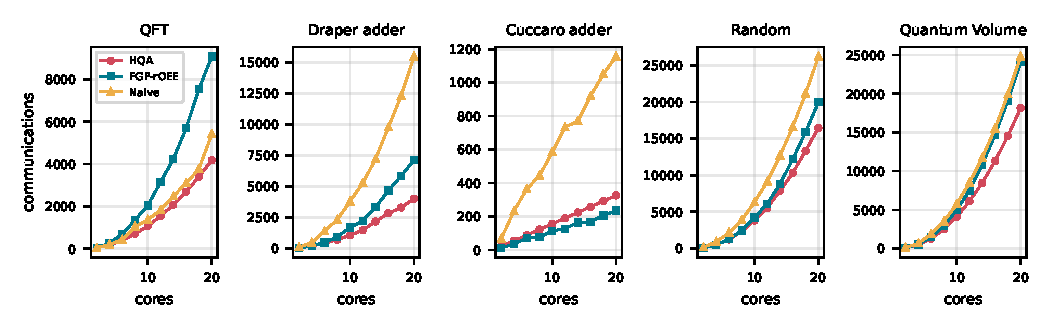
\includegraphics[width=\textwidth]{generated/fig-strong}
\caption{Strong scaling: teleportations for full cores of 10 qubits.}
\label{fig:strong}
\end{figure}

HQA needs \fgpOverHqa{} fewer teleportations than FGP-rOEE on average and
maps \hqaSpeedup{} faster (median), in line with the published
comparison.\todo{quote the papers' own averages with their configurations}
As in the papers, the exception is the Cuccaro adder, whose gates mostly join
neighbouring qubits: there FGP-rOEE needs fewer teleportations
(\cuccaroFgpOverHqa{} of HQA's). On random circuits, HQA goes below the
papers' lower bound, which assumes that qubits only move when a gate needs
them; HQA moves them ahead of time.

\section{Sparse links between cores}
\label{sec:links}

Linking every core to every other does not scale. With cores in a line, a
ring, a grid or any connected graph, moving a qubit between cores that are
not linked takes one teleportation per link on a shortest path. We adapt
HQA's cost so that both of its terms count teleportations: the links that
$g$'s qubits cross to reach $c$, and, for the look-ahead, the links each
would cross from $c$ to meet its future partners, weighted by $2^{-(m-t)}$.
With all cores linked to all, this differs from the original cost by a
constant per gate, so HQA makes the same choices. A small cost per moved
qubit (0.01) breaks ties between moving one qubit and moving both to a core
in between, and the initial OEE groups are assigned to cores so that groups
that interact most are close.

\begin{table}[t]
\centering
\begin{tabular}{lrrr}
\toprule
Links & Uniform cost / HQA & FGP-rOEE / HQA & Naive / HQA \\
\midrule
All to all & 1.00$\times$ & 1.31$\times$ & 2.34$\times$ \\
Ring & 1.06$\times$ & 1.91$\times$ & 3.84$\times$ \\
2 $\times$ 5 grid & 1.04$\times$ & 1.60$\times$ & 3.39$\times$ \\
Line & 1.10$\times$ & 1.76$\times$ & 3.17$\times$ \\
\bottomrule
\end{tabular}

\caption{100-qubit circuits on 10 cores of 10 qubits; teleportations counted
in link hops, relative to HQA with the hop-aware cost (mean over the five
benchmarks). ``Uniform cost'' is HQA with the papers' cost, which counts
every move as one teleportation.}
\label{tab:links}
\end{table}

Table~\ref{tab:links} shows that counting hops saves teleportations: the
original cost needs \uniformGrid{} to \uniformLine{} as many, most on the
line, where distances are largest. HQA's lead over FGP-rOEE grows from \fgpAlltoall{} with all cores linked to
\fgpGrid{}--\fgpRing{} on sparse links.

\section{Routing inside the cores}
\label{sec:routing}

A mapping is not yet a circuit: inside a core, qubits are coupled in a line,
a grid or another graph. We turn a mapping into a circuit on physical qubits
in three steps.
\begin{enumerate}
\item The timeslices are grouped into \emph{epochs}, runs in which no qubit
  changes core.
\item In each epoch, each core's part of the circuit, single-qubit gates and
  measurements included, is routed with SABRE~\cite{li2019sabre}, starting
  from where the previous epoch left the core's qubits (the first epoch's
  layout comes from SABRE's forward--backward search). SABRE's extended set
  also includes the gates the core's qubits have together in the next four
  timeslices, so an epoch ends with them ready.
\item Between epochs, the qubits that change core are teleported. An
  arriving qubit takes the free slot closest to the qubit it interacts with
  next or, if that one has not arrived, the free slot with most free
  neighbours, so its partner can land next to it.
\end{enumerate}
The teleportations before a timeslice happen at once, as with dedicated
communication qubits in each core, so qubits can also exchange places between
full cores. Our tests simulate the routed circuits and check that they
compute the same state as the original. Our SABRE router alone inserts
\sabreOurs{} SWAPs over \sabreCircuits{} circuits on 20-qubit lines, $5\times5$
grids and 19-qubit heavy-hex chips, against \sabreQiskit{} for Qiskit's
\texttt{SabreLayout}.

\begin{table}[t]
\centering
\begin{tabular}{llrr}
\toprule
Chip & Method & Teleportations & SWAPs \\
\midrule
2 $\times$ 5 grid & HQA & 10193 & 13628 \\
 & FGP-rOEE & 13023 & 12411 \\
 & Naive & 17790 & 10106 \\
\midrule
Line & HQA & 10193 & 26943 \\
 & FGP-rOEE & 13023 & 25028 \\
 & Naive & 17790 & 23480 \\
\bottomrule
\end{tabular}

\caption{Totals over the five 100-qubit benchmarks on 10 cores of 10 qubits
linked all to all, with the qubits of each core coupled in a $2\times5$ grid
or a line.}
\label{tab:routing}
\end{table}

Table~\ref{tab:routing} shows a trade-off that teleportation counts hide: the
naive mapper needs the most teleportations but the fewest SWAPs, because it
moves a qubit only to meet its partner and the qubit lands next to it, while
HQA also moves qubits ahead of time. HQA still has the lowest total wherever
one teleportation costs more than \breakEven{} SWAPs, which we expect of
any hardware, since a teleportation consumes an EPR pair shared across a link
and needs a Bell measurement and classical communication. Choosing the arriving qubit's slot by its next partner
saves \slotSaving{} of the SWAPs compared with taking the first free slot, and
looking ahead across epochs saves a further \lookAheadSaving{} (any horizon
from 1 to 64 timeslices is within \horizonSpread{}).

\section{Time on links of limited capacity}
\label{sec:latency}

Counting teleportations treats them alike, but a link makes EPR pairs at a
limited rate, a few at a time. We schedule the routed circuits as soon as
possible under a simple model: every operation takes a fixed time by kind;
each link has a number of \emph{channels}, each holding one EPR pair and
making the next, in a time $t_\mathrm{EPR}$, once its pair is used; a
teleportation uses one pair per link it crosses and then takes
$t_\mathrm{tel}$ per link. We use, in units of a two-qubit gate, SWAP 3,
measurement 5, $t_\mathrm{EPR} = 10$ and $t_\mathrm{tel} = 5$; these values are
illustrative.\todo{justify or vary the timing values}

\paragraph{HQA-latency.} HQA minimizes teleportations, not the length of the
critical path. We add a delay term: HQA keeps, for every qubit, when it would
be free if gates and teleportations ran as soon as possible, and adds to
$C(g, c)$ the time by which putting $g$ in $c$ delays $g$'s start, measured
in teleportations and multiplied by a weight $\lambda$. Between moving one
qubit or the other, this moves the one that has been idle, whose
teleportation overlaps other gates. No single $\lambda$ suits every circuit:
the extra teleportations it causes lengthen circuits whose links are busy.
HQA-latency therefore maps with $\lambda \in \{0, 0.25, 0.5, 1\}$, routes and
schedules each mapping under the given timing, and keeps the fastest; since
$\lambda = 0$ is HQA, it is never slower than HQA. (Including in the delay
term how busy each link is made circuits longer, so we left it out.)

\begin{table}[t]
\centering
\begin{tabular}{llrrr}
\toprule
Links & Channels & HQA-latency / HQA & FGP-rOEE / HQA & Naive / HQA \\
\midrule
All to all & 1 & \textbf{0.94$\times$} & 1.21$\times$ & 1.64$\times$ \\
 & 2 & \textbf{0.93$\times$} & 1.00$\times$ & 1.27$\times$ \\
 & 4 & \textbf{0.93$\times$} & 0.97$\times$ & 1.06$\times$ \\
 & unlimited & \textbf{0.92$\times$} & 0.96$\times$ & 1.03$\times$ \\
\midrule
Line & 1 & \textbf{0.91$\times$} & 1.49$\times$ & 2.25$\times$ \\
 & 2 & \textbf{0.91$\times$} & 1.38$\times$ & 2.08$\times$ \\
 & 4 & \textbf{0.90$\times$} & 1.27$\times$ & 1.82$\times$ \\
 & unlimited & \textbf{0.88$\times$} & 1.20$\times$ & 1.51$\times$ \\
\bottomrule
\end{tabular}

\caption{Duration relative to HQA (mean over the five 100-qubit benchmarks)
on cores of 10 qubits coupled in a $2\times5$ grid, by how the cores are
linked and how many channels each link has. HQA-latency plans for each
number of channels.}
\label{tab:latency}
\end{table}

\begin{figure}[t]
\centering
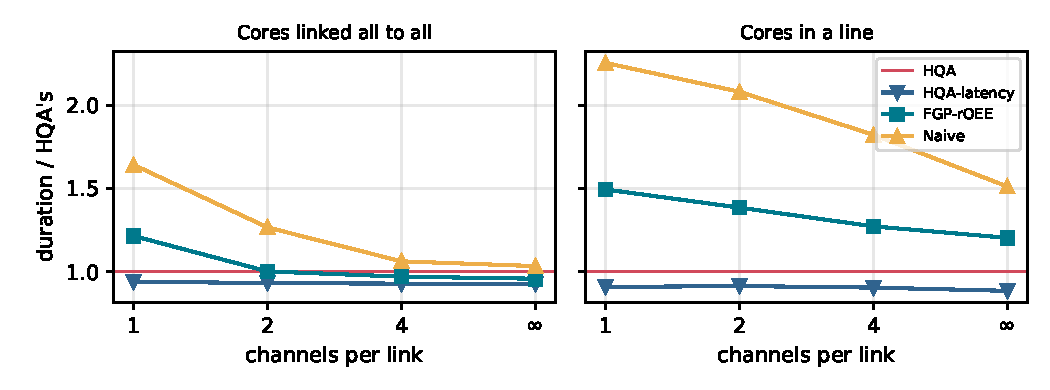
\includegraphics[width=0.85\textwidth]{generated/fig-latency}
\caption{The data of Table~\ref{tab:latency}: duration relative to HQA.}
\label{fig:latency}
\end{figure}

Table~\ref{tab:latency} and Figure~\ref{fig:latency} show two regimes. When
pairs are scarce, fewer teleportations mean shorter circuits: with one channel
per link, FGP-rOEE's circuits take \fgpSlowerOneChannelAll{} as long as HQA's
with all cores linked, and \fgpSlowerOneChannelLine{} on a line. When links
have pairs to spare, teleportations run in parallel and their number matters
less: FGP-rOEE (\fgpUnlimitedAll{}) and the naive mapper
(\naiveUnlimitedAll{}) then finish about as soon as HQA. HQA-latency is the
fastest on average in every configuration, \latencyMeanWorst{} to
\latencyMeanBest{} faster than HQA (up to \latencyBestRun{} in a single run), and
the fastest of all four methods in \latencyWins{} of the \latencyRuns{} runs,
with at most \latencyExtraTeleportations{} more teleportations than HQA. The
naive mapper remains faster on some benchmarks when links have pairs to
spare, and FGP-rOEE on the Cuccaro adder.

\section{Discussion and limitations}

The timing model ignores noise, the time to route inside a core, and the
communication qubits' own placement; durations should be read as relative.
The benchmarks are those of~\cite{escofet2025revisiting}; other circuit
families may behave differently, as the Cuccaro adder already does. Our
choices for odd core sizes and sparse links are ours, not the original
authors'. \todo{compare with further mappers from the literature (planned)}

\section{Availability}

The toolkit is MIT-licensed and installs with \texttt{pip install
qevedo-compiler}. The mappers, the router and the scheduler are in the Rust
core (\nolinkurl{core/src/multicore/} and \nolinkurl{core/src/routing/}); the
Python functions \texttt{map\_to\_cores} and \texttt{map\_and\_route} expose
them. \nolinkurl{benchmarks/multicore/run.py} and
\nolinkurl{benchmarks/routing/vs_qiskit.py} produce the results, and
\nolinkurl{paper/make.py} every table, number and figure of this paper.
\todo{cite a tagged release and archive it (e.g.\ Zenodo DOI)}

\bibliographystyle{unsrt}
\bibliography{refs}

\end{document}
